\documentclass[iop, usenatbib]{emulateapj}

%\usepackage[varg]{txfonts}
\usepackage{amssymb}
\usepackage{amsmath}
\usepackage{epsfig}
\usepackage{graphics}
\usepackage{amsmath}
\usepackage{color}
%\usepackage{xifthen}

%Debug addition for collaborators
%\usepackage[switch, displaymath, modulo]{lineno}
%\linenumbers
%%\renewcommand\linenumberfont{\color{red}\normalfont\tiny\sffamily}
%\renewcommand\linenumberfont{\normalfont\tiny\sffamily}
%\usepackage{natbib,twoopt}


%Collides with emulateapj
%%%%%%%%%
%\usepackage{siunitx}
% Units
%\DeclareSIUnit{\erg}{erg}
%%%%%%%%%


%Commands
\newcommand{\be}{\begin{equation}}
\newcommand{\ee}{\end{equation}}
%\newcommand{\bea}{\begin{eqnarray}}
%\newcommand{\eea}{\end{eqnarray}}
%\newcommand{\bea}{\begin{align}\begin{split}}
%\newcommand{\eea}{\end{split}\end{align}}
\newcommand{\ud}{\text{d}}

%normal 3-vectors
%\renewcommand{\vec}[1]{\ensuremath{\mathbf{#1}}}
\renewcommand{\vec}[1]{\ensuremath{\boldsymbol{#1}}​}

%four-vectors
\makeatletter
\def\fvec#1{\underline{\sbox\tw@{$#1$}\dp\tw@\z@\box\tw@}}
\makeatother

%higlight color
\newcommand{\red}[1]{\textcolor{red}{#1}}

%general shortcuts
\newcommand{\pd}{\ensuremath{\partial}} %partial derivative
\newcommand{\rg}{\ensuremath{r_{\mathrm{g}}}}
\newcommand{\Req}{\ensuremath{R_{\mathrm{e}}}}
\newcommand{\sch}{Schwarzschild }
\newcommand{\Ca}{\ensuremath{\mathcal{C}}}

\newcommand{\rb}{\ensuremath{\bar{r}}}
\renewcommand{\ub}{\ensuremath{\bar{u}}}
\newcommand{\wb}{\ensuremath{\bar{\omega}}}
\newcommand{\Ob}{\ensuremath{\bar{\Omega}}}
\newcommand{\nub}{\ensuremath{\bar{\nu}}}
\newcommand{\zetab}{\ensuremath{\bar{\zeta}}}
\newcommand{\Bb}{\ensuremath{\bar{B}}}
\newcommand{\mub}{\ensuremath{\bar{\mu}}}

%%%%%%%%%%%%%%%%%%%%%%


\slugcomment{ }
\shorttitle{Radiation from rotating oblate neutron stars}
\shortauthors{N\"attil\"a \& Pihajoki}

\voffset=-1cm

\begin{document}
\title{Radiation from rotating oblate neutron stars}

\author{Joonas N\"attil\"a\altaffilmark{1}\thanks{nattila.joonas@gmail.com}
and Pauli Pihajoki\altaffilmark{1}}

\affil{}
\altaffiltext{1}{Tuorla Observatory, University of Turku}

\begin{abstract}
Formulas are to be derived for gravitational bending near rotating compact objects.
\end{abstract}
\keywords{stars: neutron}

\section{Introduction}
\clearpage

%________________________________________________________________
\section{Theory}

\subsection{Space-time metrics}

\begin{table*}[ht!]
  \label{tab:coeffs}
%\renewcommand{\arraystretch}{1.4}
\begin{center}
\caption{Series expansion terms of the metric coefficients up to $\Ob^2$}
%\begin{small}
\begin{tabular}{l c c c c}
  \hline
  \noalign{\vskip 0.5ex}
              &  $\Ob = 0$  &  $\Ob^1$   & $\Ob^2$  &  error  \\
  \hline
  \noalign{\vskip 2ex}
  $\nub$       &  $\displaystyle \log\left[ 1-\frac{\ub}{2}\right] - \log\left[ 1+\frac{\ub}{2} \right]$ & --- & $\displaystyle +\left(\frac{\beta}{3}-qP_2(\cos\theta) \right)\ub^3 $ & $+\mathcal{O}\left(\Ob^2 \times \ub^4 \right)$ \\[3ex]
  $\Bb$         &  $\displaystyle \left( 1-\frac{\ub}{2} \right) \left(1+\frac{\ub}{2} \right)$ & --- & $\displaystyle+\beta \ub^2$ & $+\mathcal{O}(\Ob^4) \times \mathcal{O}(\ub^4)$ \\[3ex]
  $\zetab$     &  $\displaystyle \log\left[ \left( 1-\frac{\ub}{2} \right) \left(1+\frac{\ub}{2} \right) \right]$ & --- & $\displaystyle +\beta \left( \frac{3}{4}P_2(\cos{\theta}) - \frac{1}{3} \right) \ub^2$ & $+\mathcal{O}(\Ob^2) \times \mathcal{O}(\ub^4)$ \\[3ex]
%  $\wb$       & --- &  $\displaystyle \frac{2G\mathcal{J}}{c^2\rb^3}$ & $\displaystyle -\frac{3}{2}\ub + \mathcal{O}(\ub^2)$ & $+\mathcal{O}(\Ob^3)$ \\[2ex]
  $\wb$       & --- &  $\displaystyle \wb_1 \ub^3 $ & $\displaystyle -3\wb_1 \ub^4 $ & $+ \mathcal{O}(\Ob^3) + \wb_1 \ub^3 \times \mathcal{O}(\ub^2)$ \\[2ex]
  \hline
\end{tabular}
\begin{center}{ 
    Note:
    The angular velocity term of the local inertial frame is simplified by the notation $\wb_1 \equiv 2c^4 j/G^2 M$.
}
\end{center}
%\end{small}
\end{center}
\end{table*}


The space-time metrics of non-rotating object is given by the well known (isoradial) \sch solution
\begin{align}\begin{split}
ds^2 & = -(1-u)dt^2 + \\
     & (1-u)^{-1}dr^2+r^2(d\theta^2+\sin^2\theta d\phi^2)
\end{split}\end{align}
where $u = 2GM/c^2 r$ is the dimensionless compact factor and $r$ is the radial coordinate that is defined so that an area of a sphere is $4\pi r^2$.
This is equivalent to an alternative solution known as Isotropic \sch metric \citep[see for e.g.][]{MTW73}
\begin{align}\begin{split}
\label{eq:ISch}
ds^2 & = -\left( \frac{1-\frac{\ub}{2}}{1+\frac{\ub}{2}} \right)^2 dt^2 + \\
     & (1+\frac{\ub}{2})^4(d\rb^2 + \rb^2(d\theta^2+\sin^2\theta d\phi^2)),
\end{split}\end{align}
where $\ub=GM/c^2\rb$ and $\rb$ is the isotropic radial coordinate defined so that the circumference of a circle in this metric is $2\pi\rb$.
In this kind of isotropic metric the angles in the constant time hyperslices are represented without distortion, hence the name of the metric.
It, however, also means that angular isotropic coordinates do not faithfully represent the distances within the spheres nor does the radial coordinate correspond directly to the radial distances.
Note that from here on, we mark all variables related to the isotropic radial coordinate with bar on top.
%The relation between these two radial coordinates can be easily seen to be $r = \rb(1+\ub)^2$.

Let us now consider a rotating compact object.
In addition to the dimensionless compact factor $u(r)$ (or $\ub(\rb)$) we now need dimensionless angular velocity to describe our system
\be
\Ob = \Omega \left( \frac{\Req^3}{G M} \right)^{1/2},
\ee
where $\Omega$ is the angular velocity of a sphere with an equatorial radius $\Req$ and a mass $M$.
The metrics near a stationary axisymmetric rotating object that is asymptotically flat can be written similarly to equation \eqref{eq:ISch} in isotropic form as \citep{BW71} 
%\bea
\begin{align}\begin{split} \label{eq:BWmetric}
ds^2 & = -e^{2\nub}c^2dt^2 +
     \rb^2 \sin^2\theta \Bb^2 e^{-2\nub}(d\phi - \wb cdt)^2 + \\
     & e^{2(\zetab-\nub)}(d\rb^2 + \rb^2d\theta^2),
\end{split}\end{align}
%\eea
where $\wb$ is the angular velocity of the local inertial frame and the functions $\nub$, $\Bb$ and $\zetab$ in the metric coefficients can be expanded in the powers of $\Ob$ and $\ub$ \citep{BI76}.
The zeroth terms of the series expansions ($\Ob = 0$) are the familiar Isotropic \sch metric coefficients (see Table \ref{tab:coeffs}).
%\be
%e^{\nu_0} = (1-\ub/2)/(1+\ub/2),
%\ee
%\be 
%\Bb_0 = (1-\ub/2)(1+\ub/2)
%\ee
%and
%\be
%\zetab_0 = \log \Bb_0.
%\ee

The first order expansion in rotation ($\Ob^1$) is formally related to Kerr metric.
In this case we introduce an angular velocity term of the local inertial frame $\wb$ that accounts for the frame-dragging effects.
Up to first order, this can be defined as
\be
\wb = \frac{2c^4j}{G^2M}\ub^3,
\ee
where the dimensionless quantity $j=\mathcal{J}/M^2$ and $\mathcal{J} = I \Omega$ is the star's angular momentum with moment of inertia $I(M,\Omega)$.

Finally, the second order expansion ($\Ob^2$) correspond to the Hartle-Throne slow-rotation approximation that introduces quadrupole moments into the spacetime metric.
These second order multipolemoments can be defined via dimensionless quantities $q$ and $\beta$ that are the dimensionless moments of energy density and pressure.
\citet{aGM14} defined an approximative relation for these parameters based on their computations of rotating NSs with various different EoSs.
Due to the NS space-time being almost hairless we can parameterize these quantities with great accuracy by only using the dimensionless angular velocity $\Ob$ and compactness factor
\be
x = \frac{G M}{c^2 \Req}.
\ee
Note that both of these parameters are defined via the equatorial circumferential radius \Req.
To the lowest order, these approximations are
\be
q = -0.11 \frac{\Ob^2}{x^2},
\ee
\be
\beta = 0.4454 \Ob^2 x,
\ee
and
\be
I = \sqrt{x} (1.136 - 2.53 x + 5.6 x^2) M \Req^2.
\ee
Note also that both $q$ and $\beta$ are $\mathcal{O}(\Ob^2)$, while $I$ is $\mathcal{O}(\Ob)$.
    
It is possible to transfer between the isoradial $r$ and the isotropic $\rb$ coordinates by using the relation \citep{FIP86}
\be
r = \Bb e^{-\nub} \rb.
\ee
The relation between the two infinitesimal radial coordinates turns out to be
\be
dr = e^{\zetab} d\rb
\ee
that is calculated using the series presentation of \cite{BI76}.

Because the series expansions of the metric coefficients are expanded using the isotropic radial coordinate $\rb$ we will favor this notation in our derivation.
However, at some cases we will simplify the equations into more intuitive form by using the isoradial coordinate $r$ and so, some caution is needed when dealing with the radial coordinates.

%The metrics of the rotating isoradial spacetime is then
%\begin{align}\begin{split}\label{eq:isorad}
%ds^2 & = -e^{2\nub}c^2dt^2 +
%     r^2 \sin^2\theta (d\phi - \bar{\omega}cdt)^2 + \\
%     & e^{-2\nub}dr^2 + e^{2\mu}r^2d\theta^2),
%\end{split}\end{align}
%where $e^{2\mu} = e^{2\zetab}/\Bb^2$.
%TODO: physical explanation of the metric functions

\subsection{Oblate shape of the neutron star}

\begin{figure}
\centering
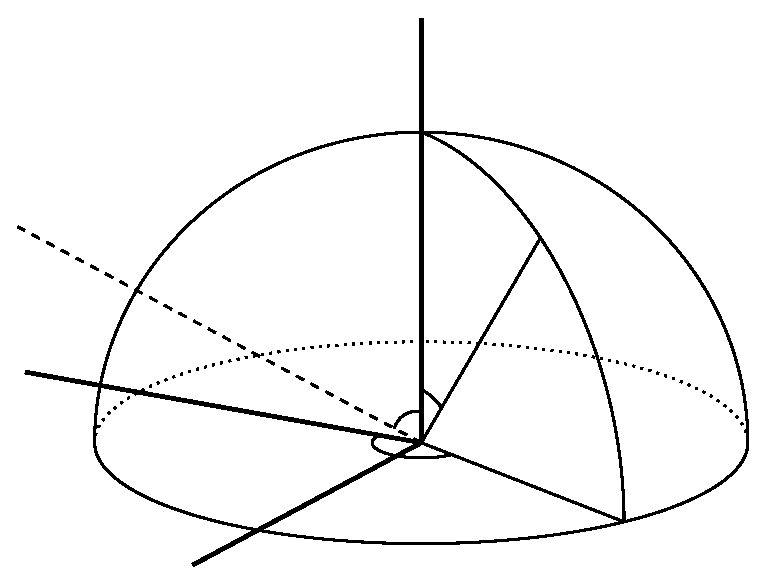
\includegraphics[width=7cm]{figs/fig1.eps}
\caption{\label{fig:geom}
  Geometry of the system.
}
\end{figure}


Due to the rotation and finite pressure supporting the system the neutron star is no longer a sphere when it is rotating.
It, however, retains the axialsymmetry and can be approximated with an oblate spheroid.
Similarly to the second order space-time quantities, \citet{aGM14} derived an approximate shape of the star as
\begin{align}\begin{split}
    R(\theta) &= \Req \left( 1 - \frac{\Req - R_{\mathrm{p}}}{\Req} \cos^2\theta \right) \\
              &= \Req (1-\Ob^2 (0.788 - 1.03x) \cos^2 \theta,
\end{split}\end{align}
where $R_{\mathrm{p}}$ is the radius on the rotational axis and $R(\pi/2) = \Req$ is the equatorial circumferential radius measured in isoradial \sch metric. 
\red{Elemental surface area for a spheroid is given as (using areal radial coordinates)
\be
dS(\theta) = R^2(\theta) \sin\theta \sqrt{1 + f(\theta)^2}d\theta d\phi,
\ee
}
where
\be
f(\theta) = \frac{1}{\bar{R}(\theta)} \frac{d \bar{R}(\theta)}{d \theta} = \Bb e^{-\zetab} e^{-\nub} \frac{1}{R(\theta)} \frac{R(\theta)}{d\theta}, 
\ee
and $\Bb e^{-\zetab} e^{-\nub} \approx (1-\frac{2 G M}{c^2 r})^{-1/2} + \mathcal{O}(\Ob^2)$.


The angle $\gamma$ defined as the angle between the radial unit vector $\vec{r}$ and the surface normal $\vec{n}$ is given by
\be
\cos\gamma = (1 - f(\theta)^2)^{-1/2}.
\ee
Then the normal to the surface can be defined using the radial vector $\vec{r}$ and the tangential vector $\vec{\theta}$ as
\be
\vec{n} = \cos\gamma \vec{r} + \sin\gamma \vec{\theta}.
\ee

See also Fig.~\ref{fig:geom} for a clarification of the angles.

\subsection{Geodesic motion through Hamilton-Jacobi equation}
Geodesic motion in space-time characterized by a metric function $g^{ij}$ is governed by Hamilton-Jacobi equation
\be
2\frac{\pd S}{\pd \tau} = g^{ij} \frac{\pd S}{\pd x^i}\frac{\pd S}{\pd x^j},
\ee
where S denotes the Hamilton's principal function.
For the two Killing vectors $k^{\alpha} = (1,0,0,0)$ (asymptotic time symmetry) and $k^{\alpha} = (0,0,0,1)$ (rotation symmetry along azimuthal angles) in the rotating space-time, the Frobenius theorem implies the existence of a family of 2-surfaces orthogonal to them.
This means that there are surfaces of constant $t$ and $\phi$ in our space-time i.e. constants of motion.
These constants are named to be $E$ and $L_z$, respectively.
We then seek a solution in the form
\be
S = \frac{1}{2}\delta_1 \tau - Et + L_z\phi + S_{\rb}(\rb) + S_{\theta}(\theta).
\ee
With the metric function \eqref{eq:BWmetric} this becomes
%\begin{align}\begin{split}
%2 r^2 \delta_{1} =~ & e^{2\nub} r^2 \pd_r^2 - e^{-2\nub} r^2 (E-L_z \omega)^2 \\
%& + e^{-2\mu} \pd_\theta^2 + \frac{L_z^2}{\sin^2 \theta},
%\end{split}\end{align}
\begin{align}\begin{split} 
    \delta_1 \rb^2 \Bb^2 e^{-2\nub} =~& \rb^2 \Bb^2 e^{-2\zetab} \pd_{\rb}S_{\rb}S^2 - e^{-4\nub} \Bb^2 \rb^2 (E - L_z \wb)^2 \\
                                & + \Bb^2 e^{-2\zetab} \pd_{\theta}S_{\theta}^2 + \frac{L_z^2}{\sin^2\theta}.
\end{split}\end{align}
After re-organizing the terms and using a simplifying notation $e^{\zetab}/\Bb \equiv e^{\mub}$ we find
\begin{align}\begin{split}\label{eq:S}
& e^{-2\mub}\pd_{\theta}S_{\theta}^2 + \frac{L_z^2}{\sin^2\theta} = \\ 
& \Bb^2 e^{-2\nub}\rb^2 ( e^{2(\nub-\zetab)} \pd_{\rb}S_{\rb}^2 -\delta_{1} - e^{-2\nub}(E - L_z \wb)^2,
\end{split}\end{align}
%By using the isoradial coordinate $r$ and notation $e^{\zetab}/\Bb \equiv e^{\mu}$ this can be simplified to
%\begin{align}\begin{split}
%    \delta_1 r^2 &- e^{2\nub} r^2 \pd_rS^2 \\
%                &+ e^{-2\nub} r^2 (E+L_z \wb)^2 = e^{-\mu} \pd_{\theta}S^2 + \frac{L_z^2}{\sin^2\theta},
%\end{split}\end{align}
that already hints towards separability if $\nub = \nub(\rb)$, $\Bb = \Bb(\rb)$, $\zetab = \zetab(\rb)$ and $\mu = \mu(\theta)$.
For the first order in rotation (i.e. $\mathcal{O}(\Ob)$) this condition is satisfied exactly because $e^{\mub} = 1 + \mathcal{O}(\Ob^2)$.
In the next order of the expansion, mass and pressure quadrupole moments are presented and so our separation is no more valid.
\red{TODO: add discussion about the higher order multipolemoments and how the deviations are rather small. for light propagation} 
%However, the deviations are rather small and for $\mathcal{O}(\Ob^2)$ pressure(?) quadrupole moment is negliblible after which we are left with  mass quadropole moment only.
%In this case the dependence of $r$ and $\theta$ are present through $e^{\nub}$ terms but $e^{\mu} \approx 1$ still.
Notice also that because we only consider null geodesics i.e. light propagation we could happily set $\delta_1 = 0$ but we choose to keep it around a bit longer to favor generality.

If we now assume separability, we can introduce a separation variable $\Ca$ known as Carter's constant (third constant of motion) in order to solve the differential equation \eqref{eq:S}.
By noting that the conjugate momenta correspond to the first derivative of $S$, with respect to the generalized coordinates we can write the general four-momentum \fvec{p} components to be
\begin{align}
  p_t       &= -E \\
  p_{\rb}    &= \pm e^{\zetab - 2\nub} \left( \delta_1 e^{2\nub} + (E - L_z \wb)^2 - \frac{\Ca}{\Bb^2 e^{-4\nub} \rb^2} \right)^{1/2}\\
  p_{\theta} &= \pm e^{\mub} \left( \Ca - \frac{L_z^2}{\sin^2\theta} \right)^{1/2}\\
  p_{\phi}   &= L_z.
\end{align}

From \fvec{p} it is also possible to derive the tetrad components \red{(isoradial!)}
\begin{align}
  p^{(t)} &= -p_{(t)} = -e_{(t)}^{\hat{\mu}} p_{\hat{\mu}} = -e^{\nub}p_t \label{eq:tetp_t}\\
  p^{(r)} &= p_{(r)} = e_{(r)}^{\hat{\mu}} p_{\hat{\mu}} = e^{\nub} p_r \label{eq:tetp_r}\\
  p^{(\theta)} &= p_{(\theta)} = e_{(\theta)}^{\hat{\mu}} p_{\hat{\mu}} = \frac{1}{r} e^{-\mu} p_{\theta} \label{eq:tetp_theta}\\
  p^{(\phi)} &= p_{(\phi)} = e_{(\phi)}^{\hat{\mu}} p_{\hat{\mu}} = -e^{-\nub} \wb p_t + \frac{1}{r \sin\theta} p_{\phi} \label{eq:tetp_phi},
\end{align}
where \red{XXX}.


\subsection{Ray tracing photons}
Radiation is emitted from the surface of a star at an emission point $(r_e,\theta_e,\phi_e)$. 
The radiation travels along a geodesic with a spectral radiance $I_{\nu}$ as measured by an observer co-moving with the emission point.
The radiation is observed at an image plane situated at a radial distance $r$, with $r\rightarrow\infty$.
We then wish to calculate the projected image of the star at this image plane.

First we set up the coordinate system so that the plane of observation is towards $\phi = 0$ and $\theta = i$, where $i$ is the angle of inclination.
The geodesic will be emitted with a four-momentum $\fvec{p}_e$\footnote{Or four-velocity $\fvec{u}_e$ as we are dealing with photons without rest mass}, and if it is eventually observed at the image plane at infinity, it will have a final four-momentum of $(E,\hat{p_r},0,0)$, purely in the radial direction.
Likewise, the components of the position must satisfy
\begin{align}
\theta &\rightarrow i \\
\phi   &\rightarrow 0,
\end{align}
as $r\rightarrow\infty$.
The total change in the angular components along the geodesic can be written as
\begin{align}
\Delta\theta &= \int_{r_e}^\infty \frac{p^\theta}{p^r}\ud r \label{eq:deltatheta} \\
\Delta\phi   &= \int_{r_e}^\infty \frac{p^\phi}{p^r}\ud r \label{eq:deltaphi},
\end{align}
so the condition for being observed is
\begin{align}
\theta_e + \Delta\theta &= i \label{eq:thetacond}\\
\phi_e + \Delta\phi     &= 0 \label{eq:phicond}.
\end{align}

The projected image of the star on the image plane can then be described by two celestial coordinates:
abscissa $\hat{x}$ and ordinate $\hat{y}$.
Making use of the tetrad components (\ref{eq:tetp_t} - \ref{eq:tetp_phi}) we obtain \red{(isoradial!)}
\be\label{eq:xhat}
\hat{x} = \left( \frac{rp^{(\phi)}}{p^{(t)}} \right)_{r \rightarrow \infty} = \frac{1}{\sin i} \frac{L_z}{E}
\ee
and
\be\label{eq:yhat}
\hat{y} = \left( \frac{rp^{(\theta)}}{p^{(t)}} \right)_{r \rightarrow \infty} = \frac{\sqrt{\Ca - \frac{L_z^2}{\sin^2 i}}}{E}.
\ee

From here it is intriguing to chance into polar coordinate system $(b, \chi)$ as the form of the equations \eqref{eq:xhat} and \eqref{eq:yhat} strongly suggest a more intuitive form if done so.
In this new coordinate system we can define the radial distance from the center point, or the impact parameter $b$, and a rotation angle $\chi$.
We will take $\chi$ to increase clockwise from the projected spin axis of the neutron star, with $\chi=0$ corresponding to the projected direction from the south to the north pole of the neutron star.
We can then express the impact parameter $b$ and the angle $\chi$ via the constants of motion of the geodesics, the $z$-component of the angular momentum, $L_z$, and the Carter constant $\Ca$, at the image plane as
\be
b = \frac{\Ca^{1/2}}{E}
\ee
and
\be
\cos \chi = \frac{1}{\sin i} \frac{L_z}{\Ca^{1/2}}.
\ee

The constants of motion, combined with the geodesic null condition $p^\mu p_\mu = 0$, allow us to solve $p^\theta$ and $p^\phi$ in terms of $r$.
We can then substitute these back into equations \eqref{eq:thetacond} and \eqref{eq:phicond}, to get the implicit solutions for $b$ and $\chi$ as
\begin{align}
\theta_e + \Delta\theta &= \Theta(R_e, \theta_e, \phi_e, b, \chi) = i\\
\phi_e + \Delta\phi     &= \Phi(R_e, \theta_e, \phi_e, b, \chi) = 0.
\end{align}

Now as a final step we can substitute the four-momentum components and image-plane coordinates into \eqref{eq:deltatheta} and \eqref{eq:deltaphi} to obtain (in isoradial form and setting $E=1$ in the final expressions)
\begin{align}\begin{split}
%\int_{\mathrm{R_e}}^{\infty} \frac{p^{\phi}}{p^r} dr =
 \Delta \phi &= 
 \int_{\mathrm{\bar{R}_e}}^{\infty} \frac{ \frac{L_z}{\sin^2\theta} - e^{-2\nub}r^2\wb(E-L_z \omega)}{r^2 \sqrt{(E-L_z\omega)^2-\frac{\mathcal{C}}{e^{-2\nub}r^2}}} dr \\
 &= \int_{\mathrm{\bar{R}_e}}^{\infty} \frac{dr}{r^2} \frac{\frac{\cos\chi \sin i}{\sin^2\theta} - e^{-2\nub}r^2\wb \left(\frac{1}{b} + \wb \cos\chi \sin i \right)}{\sqrt{\left(\frac{1}{b} + \wb \cos\chi \sin i \right)^2 - \frac{1}{e^{-2\nub} r^2}}}
\end{split}\end{align}
and
\begin{align}\begin{split}
%\int_{\mathrm{R_e}}^{\infty} \frac{p^{\theta}}{p^r} dr =
    \Delta \theta &=
    \int_{\mathrm{\bar{R}_e}}^{\infty} \frac{e^{-\mu}\sqrt{\mathcal{C} - \frac{L_z^2}{\sin^2\theta}}}{r^2\sqrt{(E-L_z\omega)^2-\frac{\mathcal{C}}{e^{-2\nub}r^2}}} dr \\
    &= \int_{\mathrm{\bar{R}_e}}^{\infty} \frac{dr}{r^2} \frac{e^{-\mu} \sqrt{1-\left(\frac{\cos\chi \sin i}{\sin\theta}\right)^2}}{\sqrt{\left(\frac{1}{b} + \wb \cos\chi \sin i \right)^2 - \frac{1}{e^{-2\nub} r^2}}}.
\end{split}\end{align}
Both expression reduce back to familiar bending equations in (isoradial) Schwarzschild metric when $\wb=0$, $\sin i = 1$ and $\cos\chi = 0$ for $\Delta\theta$ expression or $\cos\chi = 1$ for $\Delta\phi$.
However, with oblate stars it suffices to notice that the previous equations are further complicated by the fact that $\bar{R}_e = \bar{R}_e(\theta)$ and $\wb = \wb(\rb, \theta)$.

\subsubsection{Emission angle $\alpha$}
The general coordinates of a photon are defined as $x^{\alpha} = (x^{t}, x^{r}, x^{\theta}, x^{\phi})$ and the four-velocity is obtained from $dx^{\alpha}/d\lambda$ through affine parameter $\lambda$.
This general photon can then be compared to a photon moving along the surface normal $\vec{n}$ to obtain the emission angle $\alpha$ in some radial distance $R$.
Four-velocity of this photon is then $w_{\alpha} = (-e^{2\nub-\zetab}, \cos\gamma, \sin\gamma, 0 )$ obtained from the standard normalization $w^{\alpha}w_{\alpha} = 0$.
The angle between the two photons also depends on the observer.
The four-velocity of a stationary distant observer is at rest compared to the object so it must move along the time-like Killing vector.
By setting this four-velocity to be $v^{\alpha}=(t_0,0,0,0)$ and using the the time-like geodesic condition $v^{\alpha} v_{\alpha} = -1$ we obtain 
\be
t_0 = \frac{e^{-\nub}}{\sqrt{1 - \Bb^2 e^{-2\nub} \rb^2 \omega^2}}.
\ee
The angle between the two photons $u^{\alpha}$ and $w^{\alpha}$ is then \citep{PFC83}
\be
\cos \alpha = 1 + \frac{u^{\alpha}w_{\alpha}}{(v^{\beta} u_{\beta})(v^{\gamma} w_{\gamma})},
\ee
originating from the inner product of the photons in the local 3-space around the observer.%
\footnote{
The aforementioned generalized vector product for photons can be obtained by considering the projection operator $h_{\alpha \beta} = g_{xx}g^{xx} + v^xv_x$.
}
The emission angle is then
\begin{align}\begin{split}
&\cos \alpha = 1 + (1-\Bb^2 e^{-2\nub} \rb^2\wb^2\sin^2\theta) \times \\
&\{ (E-L_z \wb) + e^{2\nub-\zetab} (\cos\gamma p_{\rb} + \sin\gamma B^2 \rb p_{\theta}) \}.
%&[ (E-L_z \wb) + \cos\gamma \sqrt{(E-L_z \wb)^2 - \frac{\Ca}{\Bb^2 e^{-4\nub} \rb^2}} \\
%&+\Bb e^{2\nub} \rb \sin\gamma \sqrt{\Ca - \frac{L_z}{\sin^2\theta}} ]
\end{split}\end{align}
Here it suffices to notice that we are only interested in the emission angle value at the surface of the star i.e. $\rb = R(\theta)$.

\subsection{Method of solution}
There are two fundamentally different ways to make the ray tracing:
\begin{enumerate}
\item We can either follow photons from the image plate to the star i.e. define $(b,\chi)$ (and so also get $\cos\alpha$ immediately for flux calculation) and obtain ($\theta_e,\phi_e$).
\item or we can follow the null geodesics from the surface of the star to the image plate i.e. define ($\theta_e,\phi_e$) and obtain $(b, \chi)$ and $\cos\alpha$.
\end{enumerate}

\red{
First method should be doable already by evaluating the integrals of $\Delta\theta$ and $\Delta\phi$ with some initial guess of $\theta_e$ and then iterating for solution.
This is not however, very elegant solution and it turns the problem back into numerical nuisance so why not use full numerical ray-tracing at the first place.
}

\red{
I like the second method more because then it could serve as a good analytic approximation for many not so exact ray-tracing needs (like getting a picture and lightcurve of some hotspot).
Also many real-world applications have coordinates defined on the surface of the star and then one is interested on how the photons trajectories will bend when coming to observer.
This however means that one should somehow be able to solve the integrals explicitly and solving for $(b, \chi)$.
I have tried couple of different expansions and it is at least possible to get expressions for the first order in rotation ($\Ob^1$).
This is not, however, very cool because according to Arizona group it is the quadropole moments that affect the image most.
}

%%%%%%%%%%%%

%\section{Conclusions}
\section*{Acknowledgments}

\bibliographystyle{apj}
\bibliography{allbib}

%\begin{thebibliography}
%\end{thebibliography}

\end{document}

\appendix

\section{Additional stuff about elliptic integrals and so on}

After separating the equations with the help of the Carter constant $\Ca$ we get the remaining four-momentum components to be
\be\label{eq:pr}
p_r = \pd_r S = e^{-2\nub} \left( (E-L_z \omega)^2 - \frac{\mathcal{C}}{e^{-2\nub} r^2} \right)^{1/2} = \mathcal{R}(r)
\ee
and
\be\label{eq:ptheta}
p_{\theta} = \pd_{\theta} S = e^{\mu} \left( \mathcal{C} - \frac{L_z^2}{\sin^2 \theta} \right)^{1/2} = \Theta(\theta).
\ee
Also, now in addition to our pre-defined constants $E$ and $L_z$ we get a new constant of motion thanks to $\mathcal{C}$ that leads to
\be
\frac{\pd S}{\pd \mathcal{C}} = \frac{1}{2} \int^r \frac{1}{\sqrt{\mathcal{R}}} \frac{\pd \mathcal{R}}{\pd \mathcal{C}} dr + \frac{1}{2} \int^{\theta} \frac{1}{\sqrt{\Theta}} \frac{\pd \Theta}{\pd \mathcal{C}} d\theta = 0.
\ee 
After substitution and cancellation of terms the relation leads to elliptic integrals of the form
\begin{align}\begin{split}\label{eq:Lz_C_rel}
 \int^r dr e^{\nub} & r^{-2} \left( (E-L_z\omega)^2 - \frac{\mathcal{C}}{e^{-2\nub} r^2} \right)^{-3/4}  = \\
& \int^{\theta} d\theta e^{\mu/2} \left(\mathcal{C} - \frac{L_z^2}{\sin^2 \theta} \right)^{-3/4}
\end{split}\end{align}
connecting our three constants of motion.
The underlying elliptic integral nature becomes more prominent when we remember that $e^{\mu} \approx 1$ (i.e. constant without $\theta$ depdendeny) yielding a more refined equation for the latter integral in \eqref{eq:Lz_C_rel} of
\be
-\frac{e^{\mu/2} L_z}{\mathcal{C} (\mathcal{C}-L_z^2)^{1/4}} [ \Pi(n; \alpha, -1)+\Pi(-n;\alpha, -1)],
\ee
where $\Pi$ is the incomplete elliptic integral of the third kind with parameters $n = \sqrt{1-L_z^2/\mathcal{C}}$ as the elliptic charasteristic and the angle $\alpha$ defined as $\sin^4 \alpha = (\mathcal{C}-L_z^2 \csc^2 \theta)/(\mathcal{C}-L_z^2))$ with elliptic modulus of $-1$.


\section{Special case: equatorial rays}
If we limit ourselves to the equatorial plane ($\theta=\pi/2$ reflection symmetry) the bending equations are simplified tremendously due to the loss of four-momentum component along the $\hat{\theta}$ direction.
The general coordinates of a photon are defined as $x^{\alpha} = (x^{t}, x^{r}, x^{\theta}, x^{\phi})$ and the four-velocity is obtained from $dx^{\alpha}/d\lambda$ through affine parameter $\lambda$.
Again, due to the two Killing vectors $k^{\alpha}$ and $m^{\alpha}$ we now set our constants directly to $u_{t} = 1$ and $u_{\phi} = b$, where $b$ is an impact parameter defined more thouroughly later on.
In the equatorial plane a dual of the four-velocity is then $u_{\alpha} = (1, u_{r}, 0, b)$.
Finally, from $x^{\alpha}x_{\alpha} = 0$ we can solve the $u_{r}$ component to be
\be
u_{r} = e^{-2\nub}\sqrt{(1-b\omega)^2 - e^{2\nub}\frac{b^2}{r^2}} 
\ee

The emission angle $\alpha$ is easily obtained by using the vector notation
\be
\tan \alpha = \frac{(u^{\phi}u_{\phi})^{1/2}}{(u^ru_r)^{1/2}}
\ee
yielding
\begin{align}\begin{split}
\cos \alpha = & 1 + (e^{-2\nub}r^2\omega^2 -1) \times \\
            & \left( 1+b\omega - \sqrt{(1+b\omega)^2 - \left(\frac{b}{e^{-\nub}r}\right)^2} \right),
\end{split}\end{align}
that reduced to 
\be
\cos \alpha = \sqrt{1-\left( \frac{b}{e^{-\nub_0}r} \right)^2},
\ee
on the limit of no rotation $\omega \rightarrow 0$ that corresponds to the solution in \sch space-time when we remeber that $e^{\nub_0} = (1-\rg/R)$.



